\chapter{Materiais e Métodos} %% Poderia se chamar 'Abordagem' também (?)
\label{Cap:modeloEspacos}

\section{Local de Experimentação}
\label{local-experimentacao}

O método desenvolvido neste trabalho, assim como os respectivos experimentos, foram  realizados no Laboratório de Pesquisa em Segurança Computacional (LaPSeC), da Universidade Estadual do Oeste do Paraná (UNIOESTE), com auxílio de um \textit{cluster} de computadores de alto desempenho (C3HPC) disponibilizado pela Universidade Federal do Paraná (UFPR) através do Centro de Computação Científica e Software Livre (C3LS).

\section{Materiais}
\label{Sec:subsecoesEspacos}

Para desenvolvimento da tarefas que envolvem a construção dos modelos de classificação, foi utilizada a linguagem Python\footnote{https://www.python.org/}, em sua versão 2.7.13. Como ferramentas auxiliares foram empregues bibliotecas desenvolvidas em Python e que possuem amplo uso na literatura. Dentre elas, citam-se: Numpy\footnote{https://numpy.org/}, Pandas\footnote{https://pandas.pydata.org/}, Keras\footnote{https://keras.io/}, Tensorflow\footnote{https://www.tensorflow.org/}, Scikit-Learn\footnote{https://scikit-learn.org/stable/}, Imblearn\footnote{https://imbalanced-learn.org/}, Multiprocessing\footnote{https://docs.python.org/2/library/multiprocessing.html}, dentre outras. Para algumas análises foi utilizados o ambiente Colaboratory\footnote{https://colab.research.google.com}, o qual trata-se de um \textit{notebook} Jupyter\footnote{https://jupyter.org/} integrado a um \textit{runtime} Python fornecido pela Google. O ambiente fornecido pelo ``Colab`` permite a escrita e execução de \textit{scripts} Python diretamente do navegador.

Devido ao grande volume de dados e necessidade de poder computacional que viabilizasse o treinamento em tempo hábil, foi utilizado um \textit{cluster} com as seguintes configurações\footnote{https://www.c3sl.ufpr.br/c3hpc/}:

\begin{itemize}
    \item 6 nodos de processamento, cada um com:
    \begin{itemize}
        \item 4 sockets Intel Xeon E5-4627 v2 @ 3.30GHz (8 núcleos por socket);
        \item 256 GB de RAM;
        \item Rede de alta velocidade InfiniBand ConnectX-3 56GbE.
    \end{itemize}
\end{itemize}

\section{Método}

Inicialmente, para fins da realização deste trabalho, realizou-se estudos das temáticas envolvidas mediante levantamento de bibliografia e trabalhos existentes na literatura. Os assuntos abordados contemplavam a área de detecção de intrusão e segurança computacional, além de fundamentos de inteligência artificial e aprendizado de máquina.

O presente trabalho está pautado no desenvolvimento e na avaliação de modelos classificadores de eventos de redes. Para tal tarefa, os classificadores são treinados mediante características extraídas de fluxos de comunicação de computadores e persistidas em uma base de dados. O processo de extração de conhecimento de bases de dados possui diversas etapas e as atividades desempenhadas em cada etapa podem ser realizadas mediante diferentes abordagens.

Diante deste contexto, nas seções seguintes são descritas as decisões tomadas e técnicas utilizadas para a realização das fases do processo de mineração de dados desempenhado no presente trabalho.




\subsection{Pré-processamento}
\label{subsec:pre-processamento}

Geralmente é necessário preprocessar a base de dados a ser utilizada para o treinamento, validação e teste dos métodos de detecção de intrusão. Essa tarefa contempla diversos aspectos, conforme mencionado no capítulo \ref{Cap:fundamentacao} na seção \ref{Sec:aprendizado} (página \pageref{Sec:aprendizado}).

A utilização de bases de conhecimento públicas é uma prática bastante comum no desenvolvimento de pesquisa científica. Dentre as bases existentes no domínio da detecção de intrusão, a CICIDS2017 foi utilizada para geração dos subconjuntos de treino e teste após uma série de operações de preprocessamento.

Primeiramente, mediante análise dos dados existentes na base CICIDS2017, observou-se a possibilidade de remoção de atributos irrelevantes e a necessidade de tratar valores faltantes e inválidos. Algumas das \textit{features} que descrevem os fluxos de redes existentes na base não possuem relevância para a tarefa de treinamento. Um exemplo é o atributo ``Timestamp``. Este atributo em específico possui valor correspondente a data e hora em que ocorreu a conexão. Relembrando o objetivo do classificador a ser construído e conhecimento sobre o domínio, é possível concluir que a data e hora em que ocorreu uma conexão não representa absolutamente nada no que concerne a tarefa de classificação deste evento em ``normal`` ou ``ataque``.

De mesmo modo, outros atributos referentes ao endereço IP das máquinas envolvidas podem ser descartadas, haja visto que são apenas identificadores e são mutáveis, fazendo que com que também não sejam de grande valia para o treinamento do modelo classificador. Neste contexto, além da \textit{feature} ``Timestamp``, foram removidos ``Flow.ID``, ``Source.IP`` e ``Destination.IP``.

Na etapa de preprocessamento também foi observada a existência de atributos que apresentavam mesmo valor para todos os exemplos existentes, tornando-os absolutamente irrelevantes para a diferenciação entre uma classe e outra das observações contidas na base. Os atributos removidos, por possuírem sempre o mesmo valor são apresentados na Tabela \ref{tab:atributos-com-mesmo-valor}:

\begin{table}[H]
    \centering
    \begin{tabular}{cc}
        \hline
        \textbf{Atributo} & \textbf{Atributo} \\
        \hline
        Bwd.PSH.Flags & Fwd.Avg.Bulk.Rate \\
        Bwd.URG.Flags & Bwd.Avg.Bytes.Bulk \\
        Fwd.Avg.Bytes.Bulk & Bwd.Avg.Packets.Bulk \\
        Fwd.Avg.Packets.Bulk & Bwd.Avg.Bulk.Rate \\
        \hline
    \end{tabular}
    \caption{Atributos que apresentam o mesmo valor para todos os exemplos existentes.}
    \fonte{Fonte: O autor.}
    \label{tab:atributos-com-mesmo-valor}
\end{table}

Sendo assim, após a remoção de todos os atributos julgados irrelevantes para o método de classificação deste trabalho, houve uma redução significativa na dimensão da base de dados original, que anteriormente possuía 85 atributos e passou a ter 72, incluindo o atributo de classe do exemplo.

Conforme visto nos capítulos anteriores, no aprendizado supervisionado a existência da classe de cada um dos elementos é essencial, pois é por intermédio da classe conhecida que é possível mensurar a capacidade de aprendizado do modelo. Na CICIDS 2017 foram observados diversos exemplos que não possuíam rótulo definido. Dentre as diferentes abordagens existentes para tratar esse tipo de problema, optou-se por removê-los do \textit{roll} de observações consideradas pelo fato deste conjunto de dados possuir grande número de observações.

Seguindo a mesma política, também foram retirados todos os eventos com valores faltantes (``NaN``, do inglês ``\textit{Not a number}``) ou inválidos, como valores infintos. A Tabela \ref{tab:remocao-exemplos} quantifica os exemplos removidos de acordo com a motivação da remoção dos mesmos.

\begin{table}[H]
    \centering
    \begin{tabular}{cc}
        \hline
        \textbf{Problema identificado} & \textbf{\# Ocorrências} \\
        \hline
        Exemplo não rotulado (sem classe) & 288602 \\
        Valor NaN em algum atributo & 1358 \\
        Valores infinitos em algum atributo & 1509 \\
        \hline
        \textbf{Total} & \textbf{291469} \\
    \end{tabular} 
    \caption{Quantidade de exemplos a serem descartados da base de dados}
    \label{tab:remocao-exemplos}
\end{table}

Em sua forma original, a base utilizada possui 15 (quinze) classes. Visto que um dos objetivos deste trabalho é a construção de classificadores binários, constatou-se a necessidade de transformar as classes, de modo que os diferentes tipos de ataques fossem agrupados e pertençam a um rótulo comum. Desse modo, criou-se uma versão binária do conjunto de dados, na qual todos os exemplos são eventos normais ou ataques, sem discriminação de qual tipo de ataque se trata. Após essa transformação, os valores possíveis para o atributo de classe passaram a ser ``BENIGN`` para eventos normais e ``ATTACK`` para eventos intrusivos.

Após as transformações desempenhadas, obteve-se um versão da base CICIDS 2017 com dimensão reduzida em termos do número de exemplos, número atributos e número de classes. A Figura \ref{fig:transformacao-cicids2017} ilustra as transformações realizadas.

\begin{figure}[!hbt]
\centering 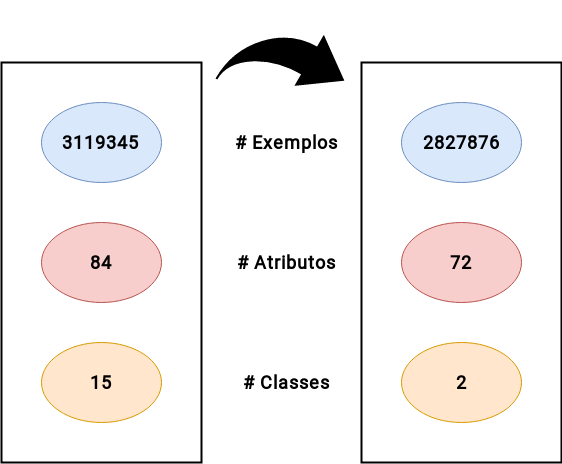
\includegraphics[width=0.8\textwidth]{{Cap4/transformacao-cicids2017.png}}
\caption{Transformação da base CICIDS2017.}
\fonte{Fonte: O autor.}
\label{fig:transformacao-cicids2017}
\end{figure}

A base de dados CICIDS2017 corresponde a registros de atributos extraídos de pacotes de rede, capturados durante a comunicação de computadores durante um período de testes, onde foram realizados diferentes tipos de ataques. Embora realizado em ambiente computacional experimental e controlado, buscou-se criar um ambiente representativo em relação ao que ocorre no mundo real. Na Tabela \ref{tab:distribuicao-classes} é possível observar a distribuição do número de exemplos pertencentes a cada uma das classes dispostas na base.

\begin{table}[H]
    \centering
    \begin{tabular}{c|cc|cc}
        \hline
        \textbf{Classe} & \textbf{\# Exemplos} & \textbf{(\%)} & \textbf{\# Exemplos} & \textbf{(\%)} \\
        \hline
        Normal & 2357511 & 83.37 & 2357511 & 83.37 \\
        \hline
        Bot & 1956 & 0.07 & \multirow{14}{*}{ 470365 } & \multirow{14}{*}{ 16.63 } \\
        DDoS & 41834 & 1.48 & & \\
        DoS GoldenEye & 10293 & 0.36 & & \\
        DoS Hulk & 230124 & 8.14 & & \\
        DoS Slowhttptest & 5499 & 0.19 & & \\
        DoS slowloris & 5796 & 0.20 & & \\
        FTP-Patator & 7935 & 0.28 & & \\
        Heartbleed & 11 & 0.00 & & \\
        Infiltration & 36 & 0.00 & & \\
        PortScan & 158804 & 5.62 & & \\
        SSH-Patator & 5897 & 0.21 & & \\
        Web Attack \textbackslash{}x96 Brute Force & 1507 & 0.05 & & \\
        Web Attack \textbackslash{}x96 Sql Injection & 21 & 0.00 & & \\
        Web Attack \textbackslash{}x96 XSS & 652 & 0.02 & & \\
        \hline
    \end{tabular}
    \caption{Distribuição de exemplos em relação a classe a que pertence}
    \fonte{Fonte: O autor.}
    \label{tab:distribuicao-classes}
\end{table}

Ao construir classificadores mediante a aplicação de algoritmos de AM, os dados fornecidos aos algoritmos de treinamento devem ser representativos em relação ao problema a ser solucionado. Entretanto, em diversas aplicações do mundo real não é possível adquirir um número de observações de classe anômala tão grande quanto de observações da classe normal, resultando em conjuntos de dados desbalanceados quanto aos rótulos dos exemplos que os compõem.

Diante do problema de desbalanceamento de classes existente nesta base, foram utilizadas técnicas para lidar com esta característica dos dados. Para o treinamento de modelos de classificação binária, buscou-se contornar a limitação do desbalanceamento por meio da aplicação de métodos de \textit{undersample} e \textit{oversample} dos exemplos existentes. \textit{Random undersampling} (ou \textit{undersampling} aleatório) foi o método escolhido para realizar a diminuição da dimensão dos conjuntos de dados de modo aleatório, diminuindo o número de exemplos da classe majoritária, enquanto o método SMOTE foi empregado na tarefa de balanceamento dos dados mediante geração de dados sintéticos baseados nos exemplos da classe minoritária.

Na Tabela \ref{tab:exemplos-apos-over-e-under}, é possível observar um comparativo da diferentes versões da base CICIDS 2017 definidas neste trabalho. Nela são apresentadas as quantidades de exemplos existentes na base original, tal como o número de exemplos existentes nas bases onde foram aplicadas as técnicas \textit{undersampling} e \textit{oversampling}. Nesta tabela, também é possível comparar a distribuição dos exemplos de acordo com a classe a que pertence, informação que explicita o desbalanceamento na base original e a correção dessa limitação nas demais bases.

\begin{table}[H]
    \centering
    \begin{tabular}{cccc}
        \hline
        \textbf{Classe} & \multicolumn{3}{c}{\textbf{\# Exemplos}} \\
        \hline
        & Original & \textit{Oversampled} & \textit{Undersampled} \\
        Normal & 2357511 (83.37\%) & 2357511 (50\%) & 470365 (50\%) \\
        Ataque & 470365 (16.63\%) & 2357511 (50\%) & 470365 (50\%) \\
        \hline
        \textbf{Total} & \textbf{2827876} & \textbf{4715022} & \textbf{940730} \\
    \end{tabular} 
    \caption{Número de exemplos após processos de \textit{oversample} e \textit{undersample}.}
    \fonte{Fonte: O autor.}
    \label{tab:exemplos-apos-over-e-under}
\end{table}

\begin{comment}
Para os dados a serem submetidos aos modelos de classificação multi-classe foi utilizada a técnica de \textit{cost sensitive training} por meio da ponderação da função de custo durante o treinamento, aplicando pesos maiores para as classes minoritárias.
\end{comment}

Ainda em relação ao processamento da base de dados, foram criados subconjuntos com redução de complexidade quanto ao número de \textit{features} utilizadas. Essa tarefa, também conhecida como seleção de atributos, pode se dar de diversas formas. É possível desempenhar a seleção de atributos através da aplicação de algoritmos capazes selecioná-los de forma automática, por exemplo, elencando as propriedades com maior ganho de informação \cite{souza2018}. Também é possível definir os atributos a serem utilizados baseando-se em conhecimento prévio acerca da área de aplicação ou por inferência baseadas em fatos observados.

Embora tenham sido criados subconjuntos de dados com dimensão reduzida quanto às \textit{features} da base, não foi utilizado nenhum método automatizado de seleção de atributos. Os subconjuntos com atributos reduzidos foram construídos com base nos resultados apresentados por \citeasnoun{sharafaldin2018}.

No que concerne a seleção de atributos, \citeasnoun{sharafaldin2018} elenca os quatro (4) atributos com maior peso para cada classe de ataque da base CICIDS2017, com exceção do ataque rotulado como ``PortScan``, para qual foram elencados apenas os três (3) atributos mais relevantes. Esta seleção de atributos resultou no total de 23 atributos, os quais são apresentados na Tabela \ref{tab:selecao-atributos}, bem como o número de ocorrências desses atributos, ou seja, para quantas classes diferentes o mesmo foi elegido como um dos melhores.

\begin{table}[H]
    \centering
    \begin{tabular}{cccc}
        \hline
        \textbf{Atributo} & \textbf{\# Ocorrências} & \textbf{Atributo} & \textbf{\# Ocorrências} \\
        \hline
        Flow.Duration & 6 & ACK.Flag.Count & 1 \\
        Total.Length.of.Fwd.Packets & 6 & Active.Min & 1 \\
        Bwd.Packet.Length.Std & 5 & Average.Packet.Size & 1 \\
        Init\_Win\_bytes\_forward & 4 & Bwd.IAT.Mean & 1 \\
        Flow.IAT.Std & 3 & Bwd.Packet.Length.Min & 1 \\
        Subflow.Fwd.Bytes & 3 & Fwd.IAT.Mean & 1 \\
        Subflow.Fwd.Packets & 3 & Fwd.PSH.Flags & 1 \\
        Active.Mean & 2 & Fwd.Packets.s & 1 \\
        Bwd.Packets.s & 2 & Init\_Win\_bytes\_backward & 1 \\
        Flow.IAT.Min & 2 & PSH.Flag.Count & 1 \\
        Fwd.IAT.Min & 2 & SYN.Flag.Count & 1 \\
        Fwd.Packet.Length.Mean & 2 & & \\
        \hline
    \end{tabular}
    \caption{Atributos com maiores pesos após processo de seleção de atributos.}
    \fonte{Fonte: Adaptado de \citeasnoun{sharafaldin2018}.}
    \label{tab:selecao-atributos}
\end{table}

Diante do exposto, após a realização das tarefas de limpeza e transformação de dados, balanceamento de classes do conjunto de dados original, mediante técnicas de \textit{undersampling} e \textit{oversampling}, e seleção de atributos, obteve-se os subconjuntos a serem utilizados no treinamento dos modelos de redes neurais artificiais. Neste ponto do preprocessamento foram criados seis (6) subconjuntos. Dos seis subconjuntos resultantes, quatro deles correspondem a um subconjunto com todos os atributos e outro com os atributos selecionados apresentados na Tabela \ref{tab:selecao-atributos} para cada uma das abordagens de transformação da amostragem de exemplos (\textit{undersapling} e \textit{oversampling}). Outros dois subconjuntos foram definidos seguindo a distribuição original dos exemplos, ou seja, mantendo o desbalanceio da base. A Figura \ref{fig:subconjuntos-cicids2017} ilustra os referidos subconjuntos.

\begin{figure}[H]
\centering 
\includegraphics[width=\textwidth]{{Cap4/subconjuntos.png}}
\caption{Processo de geração dos subconjuntos da base CICIDS2017 utilizados neste trabalho.}
\fonte{Fonte: O autor.}
\label{fig:subconjuntos-cicids2017}
\end{figure}

Por fim, aplicou-se a técnica de amostragem K-\textit{Fold Stratified Cross Validation} \cite{kohavi1995}, considerando o valor de \emph{k = 10}. Sendo assim, cada um dos subconjuntos gerados, ilustrados na Figura \ref{fig:subconjuntos-cicids2017}, foi subdividido em 10 \textit{folds} de igual tamanho, inclusive mantendo a proporção de classes, visto que adotou-se uma estratégia estratificada da técnica de \textit{cross validation}. A Figura \ref{fig:cross-validation} exibe de forma esquematizada a geração dos \textit{folds} de cada uma das bases.

\begin{figure}[H]
\centering 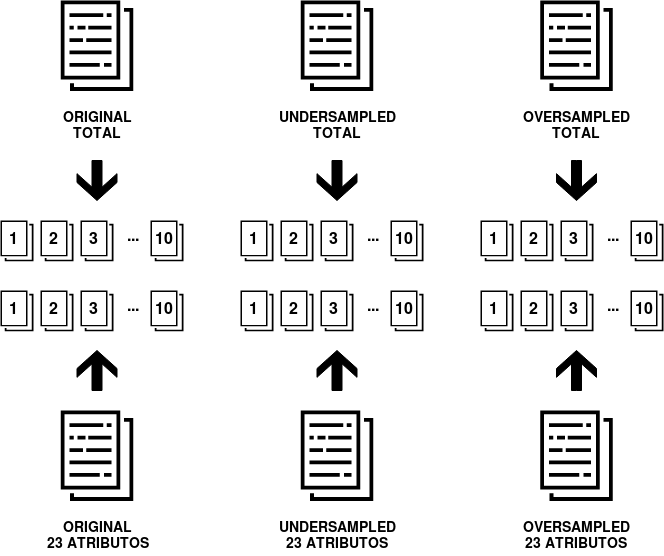
\includegraphics[width=\textwidth]{{Cap4/cross-validation.png}}
\caption{Divisão dos subconjuntos em 10 \textit{folds} para realização do \textit{Cross Validation}.}
\fonte{Fonte: O autor.}
\label{fig:cross-validation}
\end{figure}

Fazer transição entre a parte de pré-processamento e processamento.
Até aqui não ficou claro qual é o método proposto. A preparação da base direciona para os experimentos, mas quais e com qual objetivo? 


\subsection{Processamento}

O processo de treinamento de modelos de aprendizado de máquina com altos volumes de dados geralmente exige grande poder computacional e pode levar a várias horas e/ou até dias para que sejam finalizados. Neste trabalho, a fim de otimizar o tempo de treinamento e usufruir de recursos disponibilizados pelo \textit{cluster} utilizado, aplicou-se computação paralela por meio do módulo \textit{multiprocessing}, disponível no ecossistema da linguagem Python. Com isso, foi possível realizar o treinamento das diferentes configurações de redes neurais, de modo concorrente.

Os métodos de classificação foram construídos de modo supervisionado, sendo necessário treinar o modelo com parte dos dados existentes, e testá-lo com outra parte dos exemplos contidos na base de dados. Conforme mencionado na seção \ref{subsec:pre-processamento} (página \pageref{subsec:pre-processamento}), como técnica de amostragem foi utilizada a validação cruzada (\textit{cross validation}).

Esta técnica é efetuada de modo iterativo, onde os conjuntos de treino e teste são arranjados baseados nos \textit{folds} criados. O número de iterações é correspondente ao número de \textit{folds} existentes, de modo que, em cada uma das iterações, um dos \textit{folds} corresponde ao conjunto de teste, enquanto o restante dos subconjuntos compõem o conjunto de treino do modelo. Visto que neste trabalho foi definido que o número de subconjuntos é igual a dez (10), ou seja, aplicou-se um 10-\textit{Stratified-Cross-Validation}, a relação resultante desse processo é de 90\% da base sendo fornecida para treinamento e 10\% para teste. Neste caso, o produto do \textit{cross validation} é um grupo de 10 redes neurais construídas, com uma matriz de confusão correspondente a cada um dos modelos, tornando possível o cálculo das métricas de avaliação abordadas no Capítulo \ref{Cap:fundamentacao}.

\begin{figure}[H]
\centering 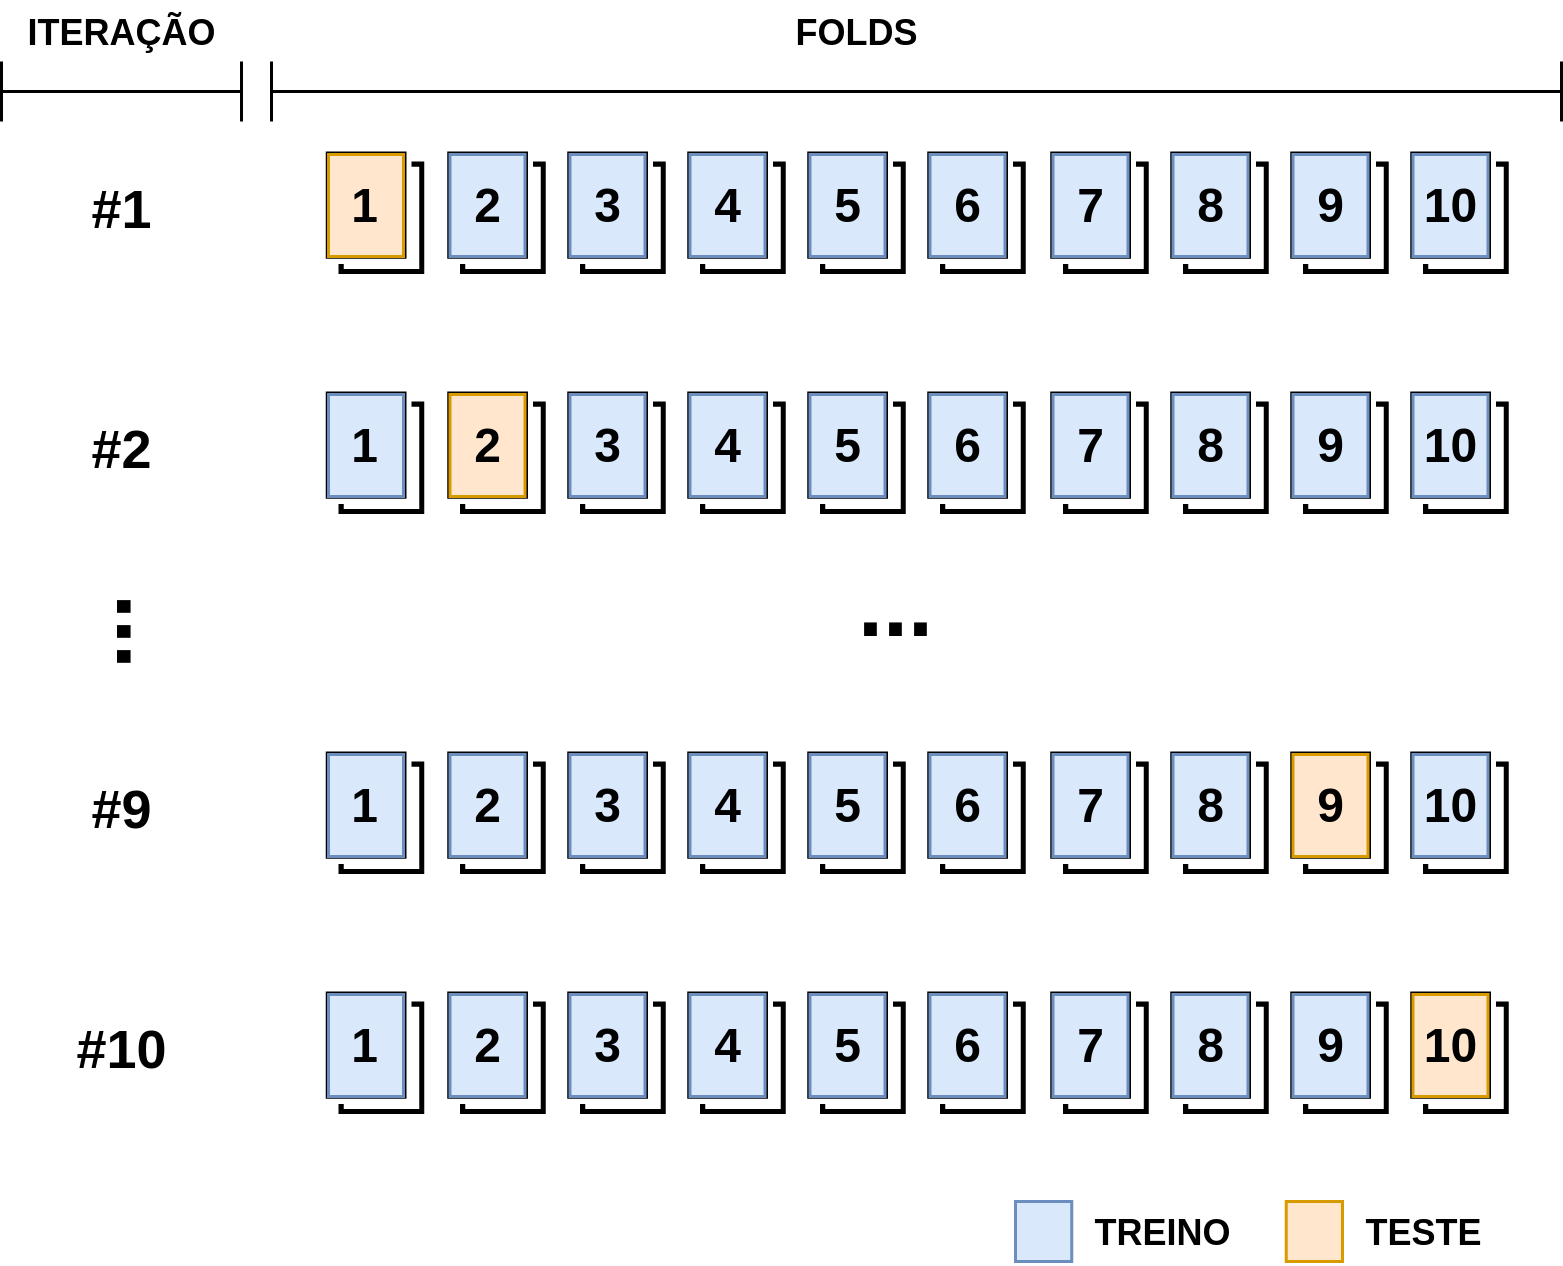
\includegraphics[width=14cm]{{Cap4/cross-validation-run.png}}
\caption{Execução da técnica de amostragem \textit{Cross Validation} para 10 \textit{folds}.}
\fonte{Fonte: O autor.}
\label{fig:cross-validation-run}
\end{figure}

Devido a características do funcionamento de redes neurais artificiais, algumas modificações nos dados são necessárias como, por exemplo, a transformação de atributos nominais para numérico. Nesta ocasião, foi necessário desempenhar essa transformação apenas no atributos de classe dos exemplos, convertendo-os de ``BENIGN`` e ``ATTACK`` para ``0`` e ``1``, respectivamente. Esse representação, tanto na forma categórica quanto na forma numérica, é conhecida como \textit{Label Encoding}.

Em seguida, os valores da classe exemplo foram também transformados para um formato de codificação conhecido como \textit{One Hot Encoding}. Assim, cada valor possível para o atributo de classe passa a ser representado como uma nova coluna na base, onde o valor será ``1`` na coluna correspondente a classe a qual o exemplo pertence, e valor ``0`` para as demais colunas. A Tabela \ref{tab:encoding} ilustra as duas diferentes representações para os mesmos exemplos hipotéticos. Para melhor entendimento, na tabela foram utilizados três possíveis valores para a classe, embora a mesma lógica seja aplicada tanto para casos binários ou multi-classe.

\begin{table}[H]
    \centering
    \begin{tabular}{cccc}
        \multicolumn{4}{c}{\textit{Label Encoding}} \\
        \hline
        \textbf{Atributo \#1} & \textbf{Atributo \#2} & \textbf{Classe Categórica} & \textbf{Classe Ordinal} \\
        \hline
        52 & 65 & Normal & 0 \\
        178 & 280 & Ataque \textit{X} & 1 \\
        164 & 347 & Ataque \textit{Y} & 2 \\
        49 & 99 & Normal & 0 \\
        26 & 58 & Ataque \textit{X} & 1 \\
        \hline
    \end{tabular}
    \begin{tabular}{ccccc}
        \\
        \multicolumn{5}{c}{\textit{One Hot Encoding}} \\
        \hline
        \textbf{Atributo \#1} & \textbf{Atributo \#2} & \textbf{Normal} & \textbf{Ataque \textit{X}} & \textbf{Ataque \textit{Y}} \\
        \hline
        52 & 65 & 1 & 0 & 0\\
        178 & 280 & 0 & 1 & 0 \\
        164 & 347 & 0 & 0 & 1 \\
        49 & 99 & 1 & 0 & 0\\
        26 & 58 & 1 & 0 & 0\\
        \hline
    \end{tabular}
    \caption{Exemplificação de diferentes formas de representação do atributo de classe.}
    \fonte{Fonte: O autor.}
    \label{tab:encoding}
\end{table}

\sigla{C.O}{Camada Oculta}

Antes de submeter os dados de entrada para iniciar o treinamento das redes neurais, os dados dos conjuntos de treino e teste são normalizados por meio do recurso disponível na biblioteca ``Scikit-Learn``. Por padrão, a biblioteca utilizada aplica a normalização L2, conhecida também como ``Distância Euclidiana``.

Durante o processo de treinamento das redes neurais, diferentes arquiteturas foram definidas e testadas no que se refere ao número de camadas ocultas (C.O) da rede. O número de camadas ocultas empregado foi variado de 1 a 5 camadas, sendo que o número de neurônios (nós) definidos para cada camada também é distinto. Para a abordagem definida com 5 camadas o número de neurônios foi de 1024, 768, 512, 256 e 128, respectivamente, da primeira para a quinta camada. Por exemplo, a estratégia que utiliza duas (2) camadas ocultas possui 1024 nós na primeira delas, e 768 na segunda. A Figura \ref{fig:arquitetura-neuronios} esquematiza a arquitetura das redes construídas quanto ao número de neurônios utilizada em cada camada oculta.

No que se refere às funções de ativação dos neurônios das redes, utilizou-se ReLU nas camadas ocultas e \textit{Softmax} na camada de saída (ambas foram mencionadas anteriormente na Seção \ref{subsec:funcoes-ativacao}, página \pageref{subsec:funcoes-ativacao}). Diante da natureza da \textit{softmax} (a qual compreende em uma distribuição de probabilidades), o número de neurônios da camada de saída é igual ao número de possíveis classes. Visto que o presente trabalho as RNA são construídas para realizar classificação binária, o número de neurônios é dois (2), conforme apresentado na Figura \ref{fig:arquitetura-neuronios}. Geralmente não aplica-se função de ativação na camada de entrada.

\begin{figure}[H]
\centering 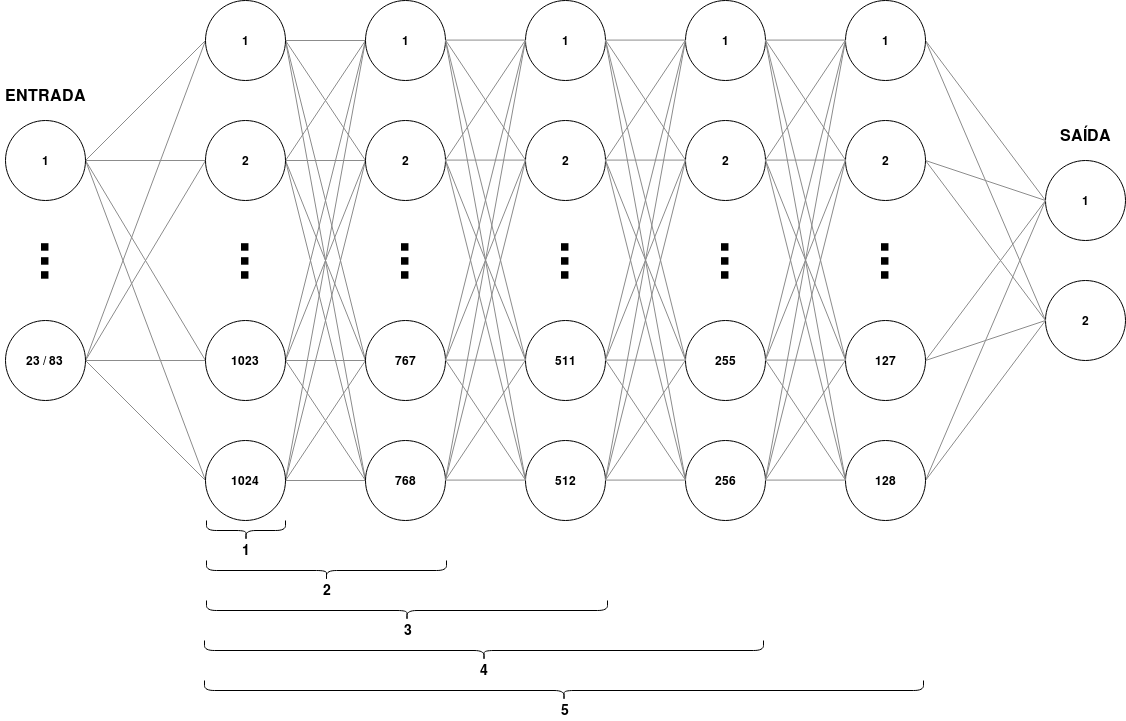
\includegraphics[width=\textwidth]{{Cap4/arquitetura-neuronios.png}}
\caption{Arquitetura das redes neurais quanto ao número de neurônios.}
\fonte{Fonte: O autor.}
\label{fig:arquitetura-neuronios}
\end{figure}

Conforme observado também na Figura \ref{fig:arquitetura-neuronios}, trata-se de uma RNA totalmente conectada, isto é, todos os neurônios de uma dada camada estão conectado com todos os neurônios da camada seguinte. De modo a aplicar a técnica de regularização da rede, a fim de diminuir as chances de ocorrência de \textit{overfitting} (quando a rede é demasiadamente ajustada para o conjunto de teste, e performa mal quando submetida ao conjunto de teste), foram incluídas camadas \textit{dropout} após cada uma das camadas ocultas.

As camadas \textit{dropout} atuam no desligamento aleatório de parte dos neurônios da rede. A probabilidade de desligamento do nó utilizada foi de 1\% em cada uma das camadas \textit{dropout}. A Figura \ref{fig:dropout} apresenta um exemplo de \textit{dropout} que resultou no desligamento de dois (2) neurônios nas camadas ocultas da rede.

\begin{figure}[H]
\centering 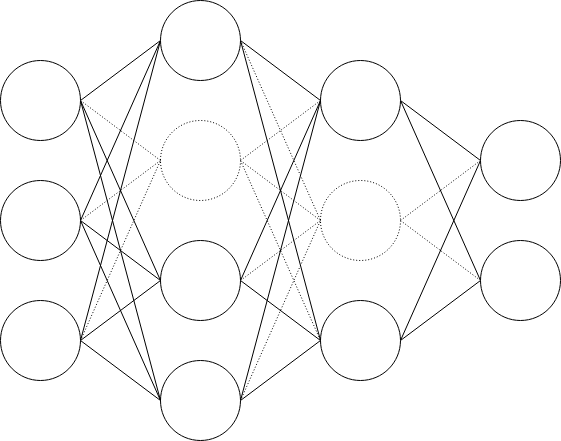
\includegraphics[width=0.8\textwidth]{{Cap4/dropout.png}}
\caption{Exemplificação da técnica \textit{dropout}.}
\fonte{Fonte: O autor.}
\label{fig:dropout}
\end{figure}

Diante do exposto na Seção \ref{subsec:treinamento} (página \pageref{subsec:treinamento}), o treinamento de uma RNA requer a definição de alguns aspectos como algoritmo de otimização, função de perda e, eventualmente, métricas a serem consideradas como mensurador de performance ou critério de parada. O algoritmo de otimização escolhido para treinamento da rede foi o Adam, com taxa de aprendizado, ou \textit{learning rate}, igual a 0.01. A entropia cruzada, ou \textit{cross entropy}, foi a função de perda escolhida.

No treinamento de uma rede neural é possível a criação de um conjunto de exemplos de validação para ser usado ao longo do processo. Na prática, o conjunto de validação é equivalente ao conjunto de teste. Porém, enquanto o conjunto de teste é destinado a avaliar o modelo apenas após a finalização do treinamento da RNA, o conjunto de validação é responsável por testar o modelo em tempo de treinamento. Desse modo, a cada época do processo de treino, é possível calcular métricas de desempenho, como acurácia ou perda, com exemplos que não foram submetidos como conjunto de treinamento, ou seja, exemplos nunca vistos pelo classificador. 10\% dos exemplos contidos no conjunto de treino foi retirado e fornecido para a validação do modelo.

O número de épocas de treino definido foi igual a duzentos (200), ou seja, são realizadas no máximo duzentas iterações em busca da convergência da rede. A fim de diminuir o tempo de execução do treino das redes, caso a mesma não esteja evoluindo de forma satisfatória, empregou-se outra técnica de regularização da rede, conhecida por parada antecipada (do inglês, \textit{early stopping}). Esta técnica consiste em monitorar uma métrica da rede durante seu treinamento, e, caso a métrica em questão não apresente melhora dentro de um período definido de \emph{x} épocas, o treinamento é finalizado. Nesta ocasião, a métrica monitorada foi a perda calculada a partir da validação do modelo, citada anteriormente, e a tolerância definida foi de vinte (20) épocas.

Por fim, após a finalização do treinamento, os conjuntos de teste (definidos conforme explicitado na Figura \ref{fig:cross-validation-run}, a qual expõe a execução do \textit{cross-validation}), foram submetidos aos modelos treinados a fim de classificá-los para posterior avaliação.

\subsection{Pós-processamento}

Na etapa de pós-processamento, utilizou-se das matrizes de confusão resultantes de cada um dos modelos construídos na fase de processamento para calcular as métricas de acurácia, precisão, \textit{recall} e \textit{f1-score}, que foram descritas na Seção \ref{Sec:avaliacao-modelos} (página \pageref{Sec:avaliacao-modelos}), com o objetivo de avaliar as arquiteturas de RNA propostas.

Além das métricas supracitas, também foi avaliado o histórico de treinamento, que consiste em métricas calculadas com base na validação dos modelos, ao longo das épocas de treinamento, conforme descrito na seção anterior.